\chapter{Structure of the project}
\thispagestyle{pagestyle}

\section{Components and features of Pie}

Pie consists of six components that serve specific purposes during the user interaction with the application. These components work independently in most of the cases, but they also have specific actions that require calling other components.

\begin{figure}[h]
\centering
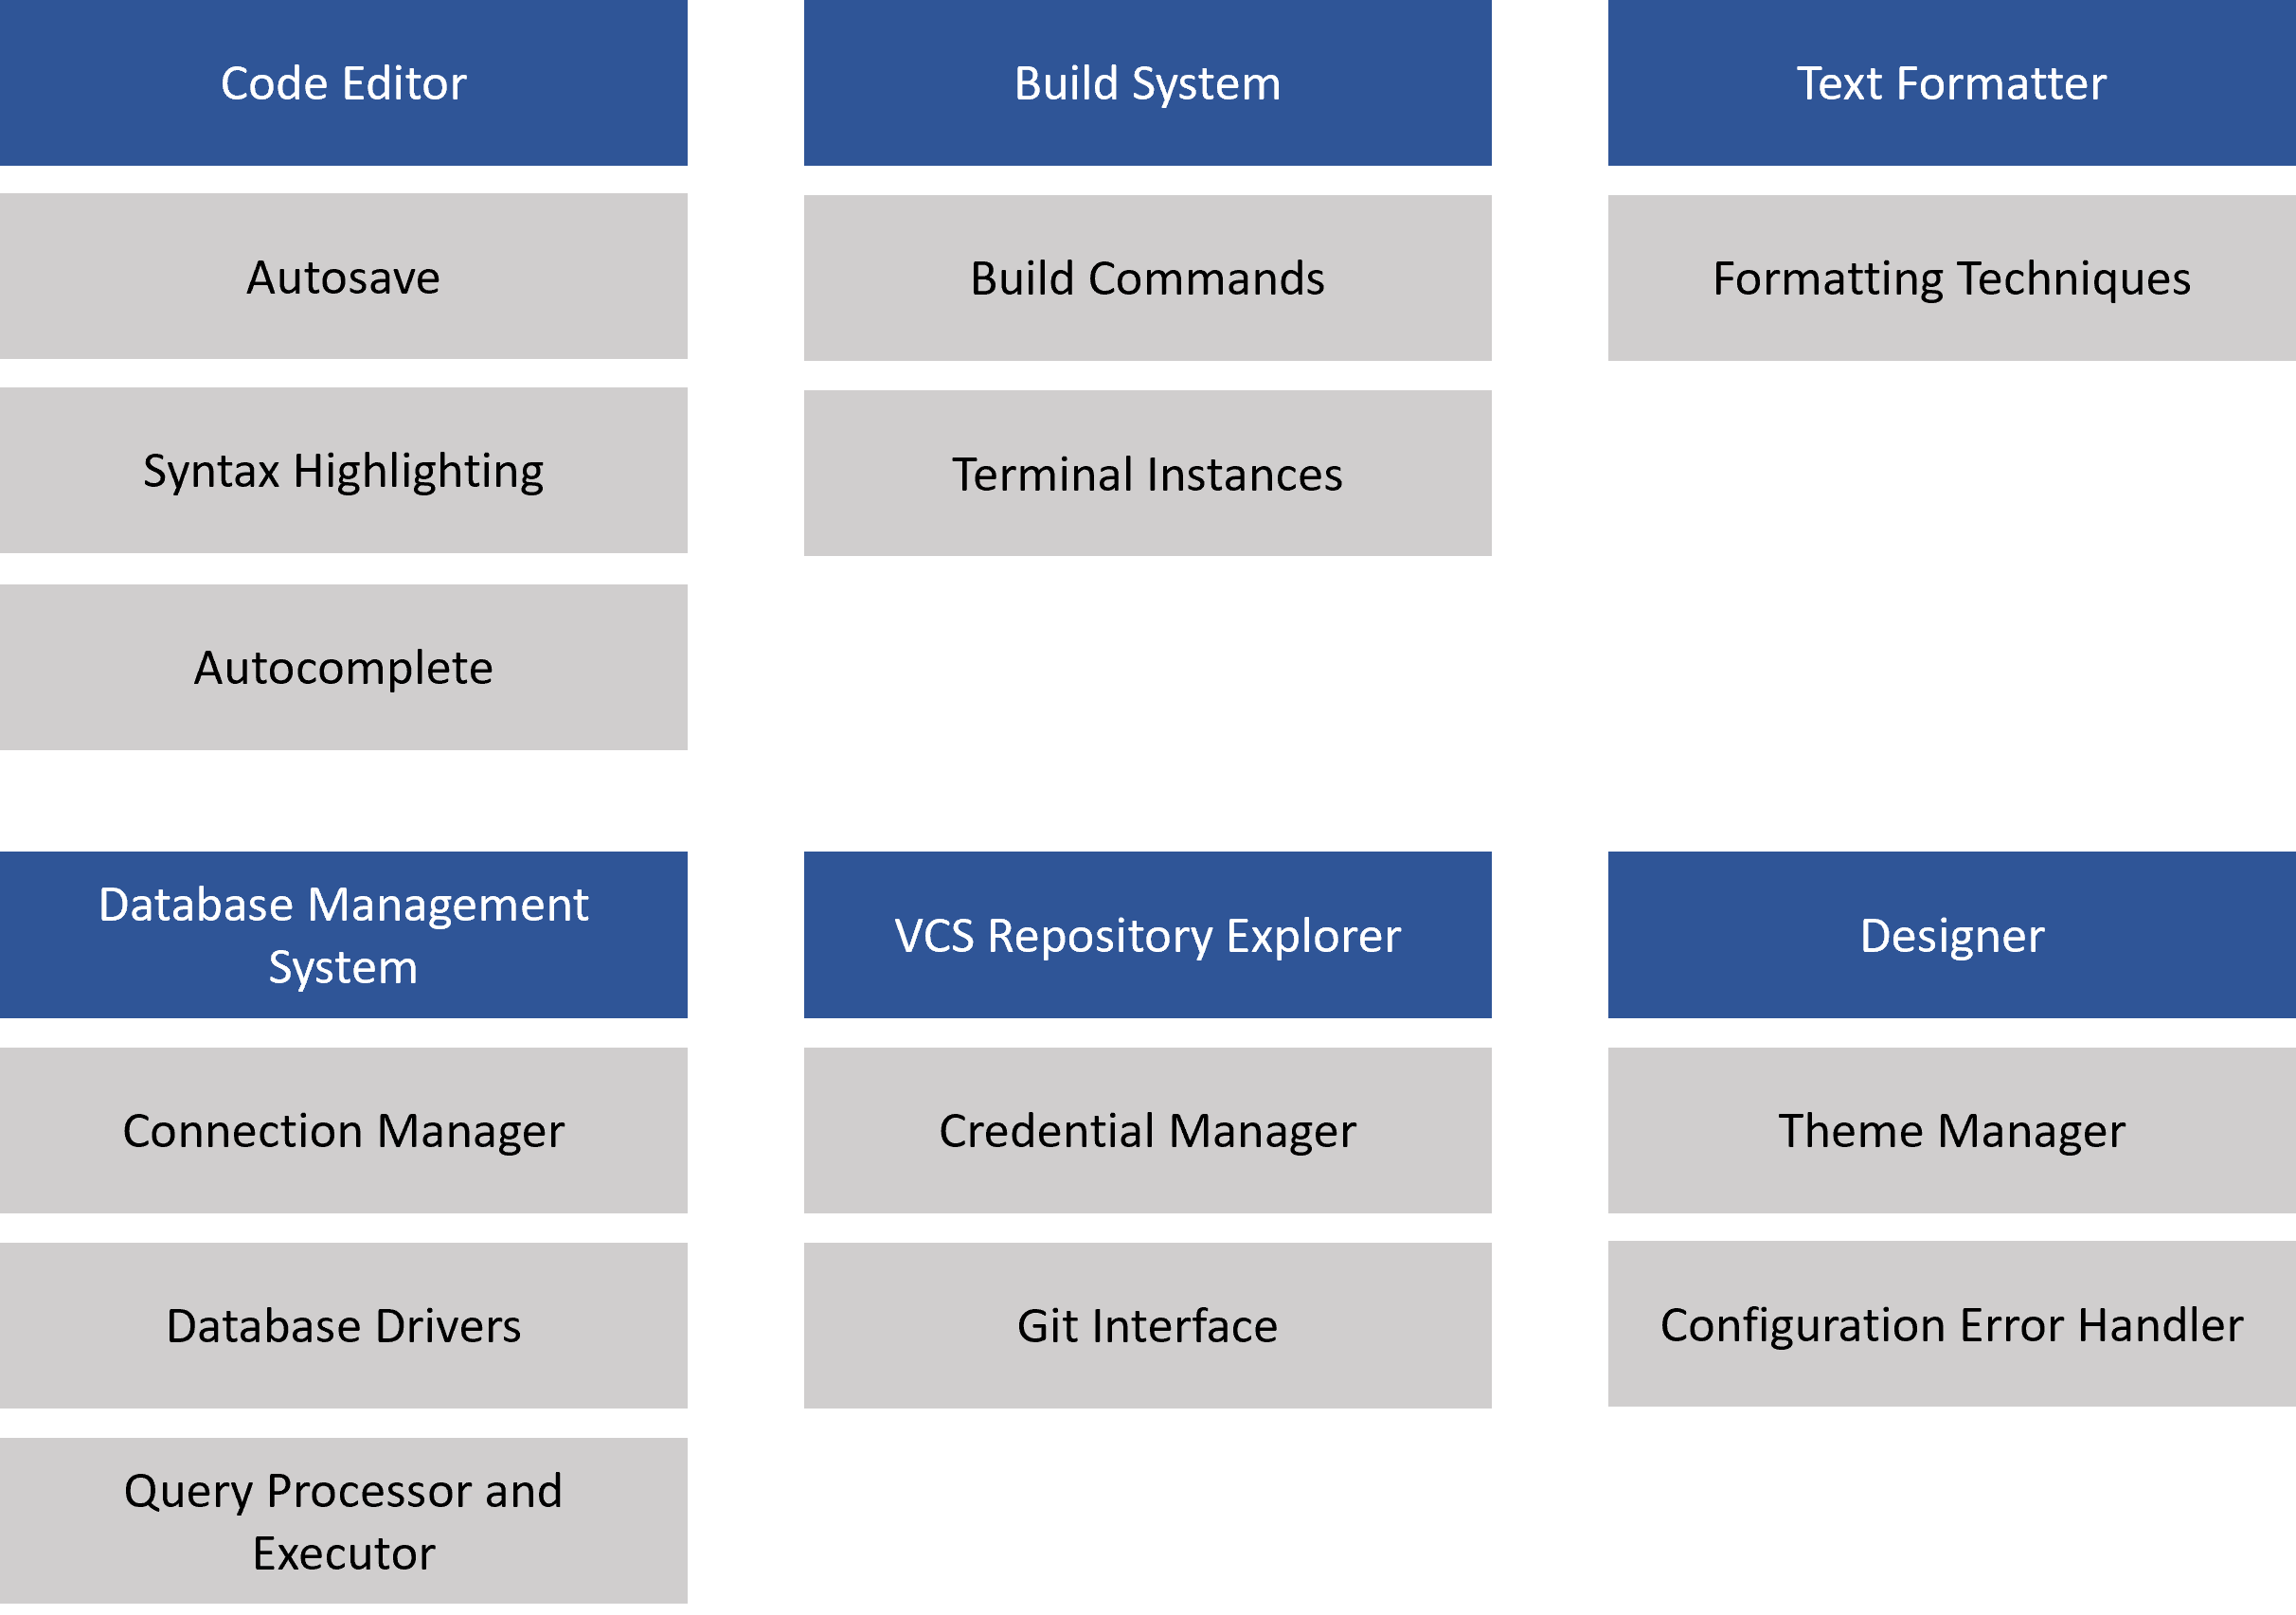
\includegraphics[width=0.6\textwidth]{images/structure.png}
\caption{The components that build up Pie}
\label{fig:fig2,1.}
\end{figure}

Code Editor provides the main capabilities of Pie. It handles the project's tab management, the instances of Scintilla, and it focuses on providing a friendly environment for the developer while writing code. The editor analyzes the extension of the opened file and initializes the syntax highlighting and autocomplete by sending a corresponding set of keywords and symbols to the Scintilla control. The component also renders HTML and Markdown files and provides proper handling of errors, when such a process fails. Going back to the independence of Pie's modules, the Code Editor works together with the Designer (component 6), when instantiating Scintilla controls, in order to provide syntax highlighting colors of the currently active theme.

The Build System allows users to add their own build commands and access them from the docked toolbar. It also handles the ConEmu terminal instances and launches every custom (or pre-defined) build command in a new terminal. Terminal tabs can also be created manually, whenever users need to input additional commands.

Text formatting capabilities were necessary, as people commonly do text-based convertions such as CSV (comma-separated values) to newline, or even backwards. Notepad++ is currently the best option for advanced text manipulation, and is often used as an extra tool during the development process, as IDEs do not provide formatting features. Pie's Text Formatter has been built for this purpose.  The tool supports common text formatting capabilities, accessible from an entire list of such actions. The list can be ordered alphabetically by the name of the formatting technique, its category or description. Users can also search through the existent actions by using the incorporated text box that updates the list in real time.

The Database Management System handles the persistence layer of Pie. It initializes a specific database connection drivers, based on several connection parameters. The connection parameters are stored in a configuration file which is read (and updated) by the manager whenever needed. This component also provides the "Run query against ..." button when a user right clicks the Scintilla control on an opened SQL file. Querying a table will result in Pie displaying a window with the output of the statement.

VCS Repository Explorer allows users to manage their local Git repositories by inspecting file statuses, viewing commit logs and pushing to/pulling from remote repositories. These actions are performed through a clean, user-friendly interface that gets opened in a new tab, whenever developers manually toggle it under the "Interface" menu element.

The Designer has influence over all of Pie's visual elements. It handles theme configuration files that can be manually added/removed by the users. The color schemes specified in the JSON-formatted data can control every aspect of the application: from the color of the windows, to the syntax highlighting color of a bracket in Scintilla. The users can also choose the theme's type: light or dark. This influences the colors of the icons (and arrows) present in Pie's controls.

\section{Architecture}

\subsection{The Model-View-Controller ("MVC") pattern}

Model-View-Controller (or "MVC") is a "pattern in software design commonly used to implement user interfaces, data, and controlling logic" \cite{mozilla-mvc}. It focuses on separating business logic from user interface code, in order to keep a cleaner project and increase its maintainability.

The MVC pattern relies on three components:

\begin{enumerate}
  \item model: defines data structures and business logic;
  \item view: defines the user interface of the application;
  \item controller: handles events, inputs and refreshes the view when needed. 
\end{enumerate}

Although this solution is a great way to separate concerns in all types of software products, including web applications where it is mostly used, Windows Forms doesn't directly implement this pattern and requires additional effort and code from the developer. I have decided not to implement it for one major reason: my code mostly relies on user interface processing. Moving logic from one place to another would result in several classes being defined only because the pattern dictates so. Entities (or models) are already defined as separate classes in Pie, so we can agree that, to a certain extent, I have integrated some aspects of the MVC pattern. However, these entities mostly resemble configuration data that is read from files or processed during the application's lifecycle.

Another advantage brought by the MVC pattern is on code testability \cite{mvc-testability}. In Pie's case, testing of business logic isn't favored because of its focus on handling user interface. It is true that several functionalities such as the Text Formatter (discussed in the next subsections) are built as input-output based services, meaning they are easy to test. However, implementing MVC over the entire application just to test several small functionalities isn't feasible. Unit testing on Pie should be done mostly on the user interface, and Microsoft already has provided solutions such as the UI Automation Framework \cite{ui-automation-framework} to do it for us.

\subsection{The file structure of the solution}

The following section describes the file structure of Pie. The application consists of a large number of C\# classes, grouped based on their purpose in folders for better readability. Figure 4.2 displays the structure of the project.

The "Forms" group consists of the windows visible to the user when interacting with the application. WinForms creates a C\# class for each Form added to the project.

"Services" typically have to do with logic that doesn't necessarily imply user interface processing. Most of the services interact with files, by performing reads and writes on them. This is how configuration data in Pie is persisted. Configuration data includes, but is not limited to, color schema definitions, database connections, and flags such as autosave and word wrap. There are several services that do more than file manipulation, such as "GitService" that calls the LibGit2Sharp API, besides handling credentials stored in .json files.

The folder named "Classes" contains the entities, commonly referred to as "models" in the MVC language. Services usually handle globally defined entities during the application runtime. For example, at the application start, the "BuildCommandService" reads all of the saved build commands from the config/build.json file and stores them in a list of "BuildCommand" objects, that is made visible when the user tries to launch a build command from the top menu strip.

"Enums" is used as a way to define types of elements. "DatabaseType" is used to convert user input (when creating a new database connection) to one of the three database management systems (MySQL, MSSQL or PostgreSQL). "TabType" has to do with the tab management system provided by the Code Editor component. A tab can be of four types: CODE, RENDER\_HTML, RENDER\_MD or GIT. This simply means that several interface elements of Pie do not open in a new window (such as the list of build commands or database connections), but they open as a new tab directly in the editor. I have implemented this, because it is more practical to switch between the tab containing the output of an HTML file and its source code, than to press a button to open a pop-up window with the output and later close it to continue with the implementation.

The "Resources" folder doesn't contain any source files or classes, but keeps icons and images used in Pie's controls. 

\begin{figure}
\centering
\framebox[0.7\textwidth]{%
\begin{minipage}{0.7\textwidth}
\dirtree{% This % is required
.1 pie. 
.2 Forms.
.3 Build Commands.
.4 AddBuildCommandForm.cs.
.4 BuildCommandsForm.cs.
.3 Databases.
.4 AddDatabaseForm.cs.
.4 DatabaseOutputForm.cs.
.4 DatabaseForm.cs.
.3 Format.
.4 FormatForm.cs.
.3 ....
.2 Services.
.3 BuildCommandService.cs.
.3 DatabaseService.cs.
.3 GitService.cs.
.3 ....
.2 Classes.
.3 GitCredentials.cs.
.3 FormatOption.cs.
.3 DatabaseConnection.cs.
.3 ....
.2 Enums.
.3 DatabaseType.cs.
.3 TabType.cs.
.3 ....
.2 Resources.
}
\end{minipage}
}
\caption{Pie's file structure, containing folders (Forms, Services, Classes, Enums, Resources) and C\# sources (*.cs)}
\end{figure}

\subsection{Event handlers in Form classes}

Pie's code mostly relies on event handling logic. Controls can also be inserted dynamically during the program's flow, besides dragging and dropping them from the toolbox. Based on events such as key presses or mouse clicks, controls are inserted, removed, shown, hidden or repositioned at runtime.